
\section{Integrated circuits structure \ddcnew}
For the purpose of properly introducing the electrical models I developed for \bbi, it is required, in the first place, to linger on how integrated circuits are structured.
It involves analyzing the main structures composing an IC, such as:
\begin{itemize}
    \setlength\itemsep{-0.1em}
    \item Its power supply network, consisting in various metal levels stacked one on top of the others;
    \item The standard-cells: pre-characterized logic cells used as elementary building blocks;
    \item The various substrate types, such as \dwF and \twF that I considered in my work, not to cite them all.
\end{itemize}

    \subsection{Power supply rails \ddcnew}
    \begin{figure}[ht]
    \centering
    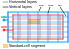
\includegraphics[width=0.45\textwidth]{3_modeling/figures/IC_POWER_PLANS.pdf}
    \caption{Coarse traditional IC power delivery diagram, showing a standard-cell segment sandwiched between power rails.}
    \label{fig:icPowerRail}
\end{figure}
    In complex digital integrated circuits, power distribution is typically realized thanks to a grid structure on multiple levels, as illustrated in Fig. \ref{fig:icPowerRail} for two metal levels.
    The upper layer forms a ring around the IC core.
    Each layer of the grid is a set of constant width metal lines equally spaced.
    The lines direction is orthogonal between layers.
    Then, vias are used to electrically connect the layers together at each overlap location.
    Commonly, the lower the layer the thinner the lines are.
    Thus, the lower grid brings the power close to each standard-cell segment, one of them being highlighted in desaturated yellow in Fig. \ref{fig:icPowerRail}.
    This topology has the advantage to bring a robust power delivery network inside the IC silicon.
    Indeed, there are multiple paths between power connections of each standard-cell segment, which leads to less power change sensitivity of the standard-cell segments.
    However, the shortcoming of such architecture lies in the high amount of metal resources required to create the power grids.

%    In most modern integrated circuits, power is brought to the transistors through various metal layers organized as meshes.
%%    The resulting meshes bring the power to the transistors, aka the logic gates, aka the Standard-Cells.
%    In digital ICs, there is typically two power delivery signals, commonly called VDD and GND, GND being the ground reference of the IC.
%    There are one or more pads for each power signal, connecting to power rings, surrounding the IC core, as shown in Fig. \ref{fig:icPowerRail}.
%    Then, power straps are created to mesh the rings and distribute evenly the power to the transistors.
%    After that, rails are drawn to connect the power to the standard-cell segments, and vias are placed between rails and straps to wire them together.

    \subsection{Standard-Cell Segments \ddcnew}
    \begin{figure}[ht]
    \centering
    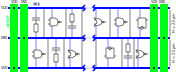
\includegraphics[width=0.55\textwidth]{3_modeling/figures/std_cell_segment_principle.pdf}
    \caption{Symbolic view of a Standard Cell Segment, surrounded by its local power delivery network.}
    \label{fig:istdCellRows}
\end{figure}
    As I described above, the power planning of ICs creates standard-cell segments (\scs), delimited by power and ground rails.
    They typically contain standard logic gates and power decoupling capacitors.
    The standard logic gates are pre-defined and pre-characterized concerning their performance (both for timing and power), for each silicon technology node, by IC manufacturers.
    They are standard in the way that their height is fixed, while their width vary according to their complexity.
    It allows placing and routing them easily in rows, delimited by the power lines around them.
    Fig. \ref{fig:istdCellRows} shows how a \scs is surrounded by VDD and GND power lines.
%    As previously mentioned, Standard-Cell Segments (\scs) are the elementary building blocks used to design ICs.
%    They are pre-defined logic cells, fulfilling a specific logic function.
%    They are pre-characterized for each technology and are used as an abstraction layer when designing integrated circuits.
%    When used in conjunction with other \scs, they allow creating a complete logic function of a portion of an IC.
%    They are usually organized in rows, with a fixed height and variable width depending on the function.
%    This allows simple power connection to each Standard-Cell Segment.
%    Fig. \ref{fig:istdCellRows} illustrates how Standard-Cell Segments are connected to the power supply network in an IC design.
%    At the top of the Standard-Cell Segment is located its VDD power input, and at the bottom its GND power input.
%    Typically, without considering various technologies, between the power rails are trapped three main regions:
%    \begin{itemize}
%        \setlength\itemsep{-0.1em}
%        \item A N-doped silicon area, called the N-well, where the PMOS transistors are lithographed;
%        \item A metal area where the transistor gates are accessible;
%        \item A P-doped silicon area, called the P-well, where the NMOS transistors are lithographed.
%    \end{itemize}
%    Therefore, NMOS transistors are located in the bottom half of the standard-cell, and the PMOS are located in the top half.

    \subsection{Various substrate types \ddcnew}
    \begin{figure}[htbp!]
    \centering
    %\scriptsize
    % \setstretch{0.9}
    \begin{subfigure}{7.8cm}
        % \def\svgwidth{9.0cm}
        \includegraphics[width=7.8cm]{3_modeling/figures/DUAL.pdf}
        \caption{Dual-Well}
        \label{subfig:dualIvx}
    \end{subfigure}
    \begin{subfigure}{7.8cm}
        % \def\svgwidth{9.0cm}
        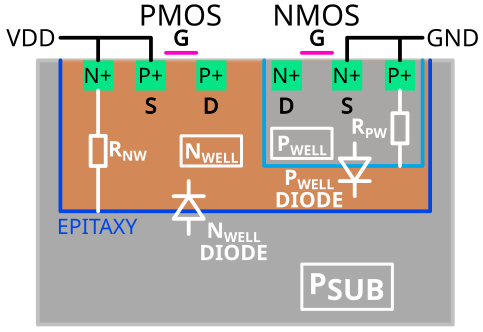
\includegraphics[width=7.8cm]{3_modeling/figures/TRIPLE.pdf}
        \caption{Triple-Well}
        \label{subfig:tripleIvx}
    \end{subfigure}
    \caption{Dual-well and triple-well inverter silicon sectional view.}
    \label{fig:dualTripleIvx}
\end{figure}
    During my work, I focused on bulk silicon substrate technologies.
    In most cases, the base silicon is P-doped, and called the substrate, on which are stacked the transistors and the power delivery network.
    In these structures, there are two typical ways of lithographing the transistors inside the silicon substrate.
    Cross-sectional views of a logic inverter manufactured with both of these techniques are shown in Fig. \ref{fig:dualTripleIvx}, and are the following:
    \begin{itemize}
        \setlength\itemsep{-0.1em}
        \item A \dwF substrate, where the NMOS transistors are lithographed into the P-doped silicon substrate, while a N-doped area called the N-well is created inside the substrate to lithograph the PMOS transistors;
        \item A \twF substrate, where an additional buried P-doped area is manufactured inside the N-well, called the P-well, allowing to lithograph the NMOS transistors inside it instead of the substrate.
    \end{itemize}
%    Now, I am going to explain the differences between \dwF and \twF substrates when modeling ICs.
%    \twF substrates offer many advantages over \dwF, such as

%    Because there are various ways to lithograph transistors for a given technology, I decided to linger and analyze the differences of two substrate types commonly found in bulk technologies:
%    \begin{itemize}
%        \setlength\itemsep{-0.1em}
%        \item \dwF substrates, where NMOS transistors are lithographed directly into the P-doped silicon substrate;
%        \item \twF substrates, where the NMOS transistors are lithographed into a buried P-well inside the N-well where the PMOS are lithographed.
%    \end{itemize}
%    For the purpose of illustrating the structural differences between those substrate types, I am going to use the schematics displayed in Fig. \ref{fig:dualTripleIvx} as a guide, illustrating the cross-sectional view of a logic inverter created in both a \dwF and a \twF substrate.

        \subsubsection{\dwF substrates \ddcnew}
        To begin with, let us focus on \dwF substrates.
        A cross-sectional view of a CMOS inverter manufactured in a \dwF substrate is shown in Fig. \ref{subfig:dualIvx}.
        Among moderately old ICs, it was common to find \dwF substrates.
        As I have stated before, in \dwF substrates, NMOS transistors are lithographed directly into the P-doped silicon substrate, as it is shown in Fig. \ref{subfig:dualIvx}.
        In addition to this, a N-doped silicon area is created inside the P-substrate, called the N-well, to lithograph the PMOS transistors.
        This results in a silicon junction, electrically represented by the N-well diode on the schematic, highlighted in saturated yellow.
        Because doped silicon does have a non-zero resistivity, electrical resistances are represented to demonstrate this:
        \begin{itemize}
            \setlength\itemsep{-0.1em}
            \item $RC_{VDD}$ represents the access resistance measured between the substrate and the PMOS transistor through the N-well;
            \item $RC_{GND}$ is the access resistance measured between the epitaxy and the NMOS transistor through the P-substrate.
        \end{itemize}

        \subsubsection{\twF substrates \ddcnew}
%        \textcolor{orange}{TW helps to reduce crosstalk noise.}
        Let us now focus on \twF substrates, which are nowadays commonly used in modern ICs because such substrates offer interesting noise properties.
        Indeed, thanks to an additional silicon well, it provides an electrical isolation between areas of the IC, thus reducing substrate crosstalk noise.

        As for \dwF substrates, the cross-sectional view of an inverter manufactured using a \twF substrate is shown in Fig. \ref{subfig:tripleIvx}.
        Similar to \dwF substrates, the PMOS transistor is lithographed in a dedicated N-well, located in the P-substrate, which creates a first diode: the N-well diode.
        Within the N-well, a P-well is created to lithograph the N-well transistor.
        Due to the appearance of a second silicon junction, it creates a second diode, the P-well diode.
        These two diodes, connected backwards relative to each other, isolate the PMOS and NMOS transistors from the rest of the substrate.
        The access resistances of these areas are:
        \begin{itemize}
            \setlength\itemsep{-0.1em}
            \item $R_{NW}$ is the access resistance between the substrate and the PMOS transistor, measured through the N-well;
            \item $R_{PW}$ is the access resistance between the N-well and the NMOS transistor, measured through the P-well.
        \end{itemize}
        It allows avoiding the propagation of switching noise from one part of the IC to another.

        Generally, \dwF and \twF substrates are used in conjunction on an IC die, therefore being able to manufacture transistors both on \dwF and \twF substrates while taking advantages of the isolating properties of \twF.

%        On the other hand, \twF substrates are also commonly used, often in combination with \dwF on the same die, to provide an electrical isolation between NMOS and PMOS transistors.
%        Thus, it helps to reduce the crosstalk noise between various areas of the IC.
%        Creating a \twF substrate is achieved by creating, inside the N-well, another doped silicon area, inversely doped, called the P-well.
%        Inside the latter are then lithographed the NMOS transistors, while the PMOS transistors are still lithographed inside the N-well.
%        This third doped area results in a second junction, which creates a second diode between the N-well and the P-well.

\section{Standard-Cell Segment (SCS) and their models \ddcu}
Thanks to what I have introduced in the previous section, that is, the Standard-Cell arrangement used to create IC architectures, alongside the two identified substrate types of interest: \dwF and \twF, it is now possible to elaborate an electrical model for such integrated circuits.
Because I am differentiating \dwF and \twF substrates, I am introducing two separate models, even though they show some similarities.
The models I developed are an improvement over the electrical models proposed by M. Dumont for \emfi \cite{mathieuEMFI}.

    \subsection{Former models \ddcnew}
    \begin{figure}[ht]
    \centering
    %\scriptsize
    % \setstretch{0.9}
    \begin{subfigure}{0.48\textwidth}
        % \def\svgwidth{9.0cm}
        \includegraphics[width=\textwidth]{3_modeling/figures/dualWellEmfi.pdf}
        \caption{\dwF model: ...}
        \label{subfig:dualScsEmfi}
    \end{subfigure}
    \hfill
    \begin{subfigure}{0.48\textwidth}
        % \def\svgwidth{9.0cm}
        \includegraphics[width=\textwidth]{3_modeling/figures/tripleWellEmfi.pdf}
        \caption{\twF model: ...}
        \label{subfig:tripleScsEmfi}
    \end{subfigure}
    \caption{Original 3-dimensional \dwF and \twF IC comprehensive Standard-Cell Segment electrical models.}
    \label{fig:dualTripleScsEmfi}
\end{figure}
    The original Standard-Cell Segment models for \dwF and \twF substrates proposed by M. Dumont \cite{mathieuEMFI} are shown in Fig. \ref{fig:dualTripleScsEmfi}.
    Let us now analyze their structure.

        \subsubsection{\dwF \scs \ddcnew}
        Fig. \ref{subfig:dualScsEmfi} shows the electrical model of an SCS for \dwF substrates.
        Each SCS is delimited by the P-substrate at its bottom (\ovalbox{1}) and by the power rails at its top (\ovalbox{5}, \ovalbox{5'}).
        The dotted wires at the bottom of the substrate indicates that each substrate layer can be repeated as required to form the correct $t_{Sub}$ thickness.
        \dwF \scs are composed of six main regions, each one describing a part of an IC core sampling:
        \begin{itemize}
            \setlength\itemsep{-0.1em}
            \item Region \ovalbox{1} is the \scs substrate resistive network, composed of six resistors;
            \item Region \ovalbox{2} is the P-substrate/N-well junction, modeled by a diode (DNW-PS) and its capacitance (CNW-PS), and is called the epitaxy, represented thanks to the blue net on the schematic. In addition to this, there is an access resistance from the epitaxy to the top of the N-well (VDD), representing the non-zero electrical resistance of N-doped silicon;
            \item Region \ovalbox{3} is the access resistance from the epitaxy up to the GND power rail, representing the non-zero electrical resistance of the P-doped substrate;
            \item Region \ovalbox{4P} is the model of the PMOS transistors, half of them being conducting. It consists in an access resistance RP from the VDD power-rail to the PMOS, and two capacitances, CGP being the load formed by the PMOS input capacitances, CGN the load formed by the NMOS input capacitances. Fig. \ref{sfig_equivCMOS} shows the model principle;
            \item Region \ovalbox{4N} is similar to \ovalbox{4P}: it is the model of the NMOS transistors, half of them being conducting. It consists in an access resistance RN from the GND power-rail to the NMOS, and two capacitances, CGP being the load formed by the PMOS input capacitances, CGN the load formed by the NMOS input capacitances. Fig. \ref{sfig_equivCMOS} shows the model principle;
            \item Region \ovalbox{5} and \ovalbox{5'} are the power network interconnections, represented on two metal levels, the colored ones being the first metal levels, the gray being the top metal level.
            \item Eventually, region \ovalbox{6} is simply the decoupling existing between both GND and VDD power rails.
        \end{itemize}

        \subsubsection{\twF \scs \ddcnew}
        Fig. \ref{subfig:tripleScsEmfi} illustrates the \scs model for \twF substrates.
        The \scs are delimited, as before, by the P-substrate at their bottom and the power delivery network at their top.
        As for the \dwF model, the bottom dotted wires indicate that each substrate layer is repeated as needed to create the correct thickness required.
        The main difference between \dwF and \twF \scs models lies in the region \ovalbox{3}.
        First, let me describe every region:
        \begin{itemize}
            \setlength\itemsep{-0.1em}
            \item As for the previous model, region \ovalbox{1} is the silicon P-doped substrate;
            \item Region \ovalbox{2} is the N-well, created inside the P-substrate, with the junction (epitaxy) represented by a blue wire. It is composed of the diode DNW-PS, and its capacitance CNW-PS, alongside the N-well access resistance RNW from the epitaxy up to the VDD network;
            \item Region \ovalbox{3} is where the \twF model drastically differ from the \dwF one. As I have explained before, in \twF substrates, the NMOS transistors are lithographed inside an isolated P-doped region called the P-well. Therefore, region \ovalbox{3} describes the P-well, with an additional silicon junction modeled with the diode DNW-PW connected backward compared to DNW-PS, its capacitance CNW-PW, and the P-well access resistance RPW to GND;
            \item The three other regions are identical to the previous \dwF model.
        \end{itemize}


%Similar to \cite{mathieuEMFI} and to VLSI design, I am using the Standard-Cells as a basic building block.
%However, in my model is not represented the logic function of a Standard-Cell, rather its electrical behavior.
%More specifically, the elementary building block of the proposed electrical model represents the average electrical behavior of several Standard-Cells, called Standard-Cell Segment (\scs).

    \subsection{Enhancing the substrate model \ddcnew}
    \begin{figure}[ht]
    \centering
    \includegraphics[width=0.65\textwidth]{3_modeling/figures/substrateSubdivision_6.pdf}
    \caption{Substrate subdivision improvement over M. Dumont model for \emfi \cite{mathieuEMFI}. The backside is the accessible substrate, and the epitaxy is the highest substrate level, a.k.a. the silicon junction between the P-substrate and the N-well.}
    \label{fig:surfaceSubDivid}
\end{figure}
    In the model designed by M. Dumont, the substrate block at the \scs bottom is only modeled thanks to six resistors.
    If it was enough to fully appreciate and simulate \emfi disturbances, it is not sufficient to model and simulate \bbi disturbances, for many reasons.

    Among them, we can identify the coarse nature of the substrate model.
    Indeed, the six resistors composing the model are sufficient in an \emfi context as the substrate acts as an almost transparent environment and is here only to create the substrate electrical interconnect between \scs.
    However, in a \bbi context, the substrate is the physical environment used to convey the energy from the metal probe to the transistors.
    In addition to this, the typical substrate thickness of ICs ranges from 40 µm to 1 mm, and using only two resistors to represent 700 µm of material is a too wide geometric step to fully appreciate the mechanisms at work during \bbi.
    Furthermore, as the modeled \scs is 5 µm wide and 30 µm long, the spatial resolution of the substrate sub model is not the same in each direction.

    Therefore, I decided to improve the former model to allow for finer geometry resolution.
    My proposition consists in fixing the width and length of an elementary substrate sub model to a value of 5 µm, while allowing the user to have a certain degree of freedom concerning the elementary thickness value.
    However, I chose a 10 µm default value for the elementary thickness as it is a good value, computationally speaking.
    To achieve this, I split the former six-resistors sub model into many six-resistors blocks connected to each other, as it is shown in Fig. \ref{fig:surfaceSubDivid}.
    These new substrate blocks then measure 5 µm by 5 µm by 10 µm.
    As one can see, to preserve the higher part of the \scs model, I kept the \scs length of 30 µm, which results in a 6 by 1 array of elementary substrate blocks.
    Eventually, these enhancements also allow me to analyze the effects of substrate thinning on the models, similar to what is done with actual ICs.

    \subsection{The considered \scs for the rest of my work \ddcnew}
    \begin{figure}[ht]
    \centering
    %\scriptsize
    % \setstretch{0.9}
    \begin{subfigure}{0.45\textwidth}
        % \def\svgwidth{9.0cm}
        \includegraphics[width=\textwidth]{3_modeling/figures/dualWell_no_5e.pdf}
        \caption{Dual-Well}
        \label{subfig:dualScs}
    \end{subfigure}
    \hfill
    \begin{subfigure}{0.45\textwidth}
        % \def\svgwidth{9.0cm}
        \includegraphics[width=\textwidth]{3_modeling/figures/tripleWell_no_5e.pdf}
        \caption{Triple-Well}
        \label{subfig:tripleScs}
    \end{subfigure}
    \caption{Three-dimensional Dual-Well and Triple-Well IC comprehensive standard-cell electrical schematic.}
    \label{fig:dualTripleScs}
\end{figure}
    Considering that the IC target I used for my experiments is the STM32F439VIT6, and because we have technical information concerning the inner structure of the target IC technology, I considered this information to calculate the various \scs model parameters.
    Therefore, every simulation presented in this work relies on a model that is as close as possible from the actual microcontroller.
    Fig. \ref{fig:dualTripleScs} presents the enhanced model used during my simulations, and Table \ref{tableValeurSimu} shows the components values calculated in accordance to the 90 nm technology.
    \begin{table}[ht]
    \centering
    \includegraphics[width=\textwidth, center]{3_modeling/figures/tableValeursSimus.pdf}
    \caption{\scs model numeric values.}
    \label{tableValeurSimu}
\end{table}


%%\begin{figure}[ht]
    \centering
    \includegraphics[width=0.65\textwidth]{3_modeling/figures/substrateSubdivision_6.pdf}
    \caption{Substrate subdivision improvement over M. Dumont model for \emfi \cite{mathieuEMFI}. The backside is the accessible substrate, and the epitaxy is the highest substrate level, a.k.a. the silicon junction between the P-substrate and the N-well.}
    \label{fig:surfaceSubDivid}
\end{figure}
%Because I based my work on M. Dumont model \cite{mathieuEMFI}, there is a common base to which I have made modifications.
%The major one consists in improving the model geometric accuracy in the case of \bbi studies.
%In M. Dumont model, the silicon P-substrate is represented solely thanks to a network of 6 resistors, 30 µm wide, 5 µm long, and $t_{Sub}$ deep, $t_{Sub}$ being the entire modeled IC substrate thickness.
%However, when performing \bbi, the substrate is the main physical environment where the electric charges travel.
%Therefore, as I describe in more details further, it is required to improve the spatial resolution of the model concerning the substrate, as shown in Fig. \ref{fig:surfaceSubDivid}.
%This is done by splitting the substrate electric model in several 6-resistors elementary networks interconnected with each other.
%It allows representing the same substrate with more resistors, thus enabling more precise analysis of the substrate charges distribution during \bbi.
%
%%\begin{figure}[ht]
    \centering
    %\scriptsize
    % \setstretch{0.9}
    \begin{subfigure}{0.45\textwidth}
        % \def\svgwidth{9.0cm}
        \includegraphics[width=\textwidth]{3_modeling/figures/dualWell_no_5e.pdf}
        \caption{Dual-Well}
        \label{subfig:dualScs}
    \end{subfigure}
    \hfill
    \begin{subfigure}{0.45\textwidth}
        % \def\svgwidth{9.0cm}
        \includegraphics[width=\textwidth]{3_modeling/figures/tripleWell_no_5e.pdf}
        \caption{Triple-Well}
        \label{subfig:tripleScs}
    \end{subfigure}
    \caption{Three-dimensional Dual-Well and Triple-Well IC comprehensive standard-cell electrical schematic.}
    \label{fig:dualTripleScs}
\end{figure}
%%%\begin{figure}[ht]
%    \centering
%    
\includegraphics[width=0.50\textwidth]{3_modeling/figures/logicGatesModelMathieu.pdf}
%    \caption{Electrical equivalent model of two inverters interconnected with each other.}
%    \label{fig_equivLogicGateStdCell}
%\end{figure}

\begin{figure}[ht]
    \centering
    \begin{subfigure}{0.52\textwidth}
        
\includegraphics[width=\textwidth]{3_modeling/figures/logicGatesModelMathieu.pdf}
        \caption{Electrical equivalent model of two inverters interconnected with each other, with the first one outputting a logical ONE value.}
        \label{sfig_equivCMOS}
    \end{subfigure}
    \hfill
    \begin{subfigure}{0.44\textwidth}
        
\includegraphics[width=\textwidth]{3_modeling/figures/stdCellLayoutSimple.pdf}
        \caption{Simplified top view of a Standard-Cell with two power rail metal levels. In blue are the logic interconnections inside the Standard-Cell.}
        \label{sfig_simpleSCS}
    \end{subfigure}
    \caption{Equivalent logic gates models used in the SCS model (\ref{sfig_equivCMOS}), and a simplified top view of a Standard-Cell with its size (\ref{sfig_simpleSCS}).}
    \label{fig_equivLogicGateStdCell}
\end{figure}
%Fig. \ref{fig:dualTripleScs} shows the complete 3-dimensional schematics of the developed models for my thesis.
%An analog simplified schematic representing the top view of a Standard-Cell is shown in Fig. \ref{sfig_simpleSCS} for understanding and clarity purposes. It describes the two levels of metal considered in my modeling (in orange and red), alongside the internal Standard-Cell interconnections in blue, with its size annotated.
%
%The next subsections are dedicated to describing these models both for \dwF and \twF substrates.
%Each SCS is 30 µm wide, 5 µm long and $t_{Sub}$ deep, the thickness of the power delivery network and the logic gates being ignored, as the substrate thickness is often big in front of the latter.
%In my models, an SCS represents about a hundred of logic gates, where half of their transistors are conducting.

%    \subsection{The case of \dwF substrates \ddcnew}
%    Fig. \ref{subfig:dualScs} shows the electrical model of an SCS for \dwF substrates.
%    Each SCS is delimited by the P-substrate at its bottom (\ovalbox{1}) and by the power rails at its top (\ovalbox{5}, \ovalbox{5'}).
%    The dotted wires at the bottom of the substrate indicates that each substrate layer can be repeated as required to form the correct $t_{Sub}$ thickness.
%    \dwF \scs are composed of six main regions, each one describing a part of an IC core sampling:
%    \begin{itemize}
%        \setlength\itemsep{-0.1em}
%        \item Region \ovalbox{1} is the substrate resistive network, composed of several resistors, and being an isotropic environment;
%        \item Region \ovalbox{2} is the P-substrate/N-well junction, modeled by a diode (DNW-PS) and its capacitance (CNW-PS), and is called the epitaxy, represented thanks to the blue net on the schematic. In addition to this, there is an access resistance from the epitaxy to the top of the N-well (VDD), representing the non-zero electrical resistance of N-doped silicon;
%        \item Region \ovalbox{3} is the access resistance from the epitaxy up to the GND power rail, representing the non-zero electrical resistance of the P-doped substrate;
%        \item Region \ovalbox{4P} is the model of the PMOS transistors, half of them being conducting. It consists in an access resistance RP from the VDD power-rail to the PMOS, and two capacitances, CGP being the load formed by the PMOS input capacitances, CGN the load formed by the NMOS input capacitances. Fig. \ref{sfig_equivCMOS} shows the model principle;
%        \item Region \ovalbox{4N} is similar to \ovalbox{4P}: it is the model of the NMOS transistors, half of them being conducting. It consists in an access resistance RN from the GND power-rail to the NMOS, and two capacitances, CGP being the load formed by the PMOS input capacitances, CGN the load formed by the NMOS input capacitances. Fig. \ref{sfig_equivCMOS} shows the model principle;
%        \item Region \ovalbox{5} and \ovalbox{5'} are the power network interconnections, represented on two metal levels, the colored ones being the first metal levels, the gray being the top metal level.
%        \item Eventually, region \ovalbox{6} is simply the decoupling existing between both GND and VDD power rails.
%    \end{itemize}

%    \subsection{The case of \twF substrates \ddcnew}
%    Fig. \ref{subfig:tripleScs} illustrates the \scs model for \twF substrates.
%    The \scs are delimited, as before, by the P-substrate at their bottom and the power delivery network at their top.
%    As for the \dwF model, the bottom dotted wires indicate that each substrate layer is repeated as needed to create the correct thickness required.
%    The main difference between \dwF and \twF \scs models lies in the region \ovalbox{3}.
%    First, let me describe every region:
%    \begin{itemize}
%        \setlength\itemsep{-0.1em}
%        \item As for the previous model, region \ovalbox{1} is the silicon P-doped substrate;
%        \item Region \ovalbox{2} is the N-well, created inside the P-substrate, with the junction (epitaxy) represented by a blue wire. It is composed of the diode DNW-PS, and its capacitance CNW-PS, alongside the N-well access resistance RNW from the epitaxy up to the VDD network;
%        \item Region \ovalbox{3} is where the \twF model drastically differ from the \dwF one. As I have explained before, in \twF substrates, the NMOS transistors are lithographed inside an isolated P-doped region called the P-well. Therefore, region \ovalbox{3} describes the P-well, with an additional silicon junction modeled with the diode DNW-PW connected backward compared to DNW-PS, its capacitance CNW-PW, and the P-well access resistance RPW to GND;
%        \item The three other regions are identical to the previous \dwF model.
%    \end{itemize}

    \subsection{Interconnecting Standard-Cell Segments together \ddcpu}
    The models I previously presented only describe a small portion of an integrated circuit, this is to say an \scs.
    Therefore, to be able to model an entire IC, it is required to instantiate several \scs and to connect them with each other in a mesh arrangement.
%    Because the \scs I previously introduced only describe a portion of an integrated circuit, in order to model a complete one, it is required to instantiate several \scs and to connect them with each other in a mesh grid.
    \begin{figure}[ht]
    \centering
    \includegraphics[width=0.5\textwidth]{3_modeling/figures/resultingSimulated_ic.png}
    \caption{Three-dimensional Standard-Cell Segments interconnection example.}
    \label{fig:surfaceSplitScs}
\end{figure}
    Fig. \ref{fig:surfaceSplitScs} shows coarsely how it is achieved.
    I have chosen to work with the SPICE simulator to perform the simulations as it is a widely used software in electronics and is available in various flavors.
    Therefore, \scs are written in SPICE language.
    As I have said before, the very elementary building substrate blocks are written manually and verified before any usage.
    Then, the \scs elementary models are automatically generated instead of being written manually.
    It allows avoiding human errors and enabling fast modifications to the models when required.

    Then comes the interconnection step.
    To that end, it is needed to create a top SPICE file which instantiates every \scs required to form the IC and defines constant parameters in addition to simulation conditions.
    I chose to use the Python language to do so as I use it for every tool I write my work, therefore enabling fast support and update, while ensuring cross-script compatibility.
%    In addition to this, I decided to create an algorithm to connect as much \scs as needed to create a resulting IC.
    By doing so, the interconnection process is automated and free from human errors.
    The actual generator Python script is annexed to the manuscript (\textcolor{orange}{TO-DO}).
    Because I have designed two separate models, one for \dwF and another for \twF substrate types, in addition to the various dynamic parameters which are useful when modeling an IC, the algorithm offers a certain degree of flexibility, allowing me to cover multiple use cases.
    The actual generation script uses procedural generation according to the input parameters.
    Various parameters are user-accessible and can be modified to fit the needs.
    Next is the list of these settings:
    \begin{itemize}
        \setlength\itemsep{-0.1em}
        \item The resulting IC size;
        \item The \bbi probe location;
        \item The IC global substrate thickness;
        \item The substrate sub-model thickness;
        \item The substrate type: \dwF, \twF, or a mix of both, allowing to replicate actual IC architectures;
        \item The voltage pulse amplitude, width, and rise and fall times;
        \item Various SPICE simulation settings.
    \end{itemize}
    Eventually, the program incorporates a visual inspection tool in order to provide a quick verification of the generated IC structure to the end-user.

    \subsection{Writing the elementary models \ddcu}
    \begin{figure}[H]
    \centering
    \includegraphics[width=0.5\textwidth]{3_modeling/figures/algoFigure5.png}
    \caption{Elementary substrate 3D netlist}
    \label{fig:algo}
\end{figure}
%    After having abstractly created the models, I decided to write them using SPICE (Simulation Program with Integrated Circuit Emphasis) language.
    If the \scs models are automatically generated, I have written manually the substrate sub models.
    Indeed, they are very simple and straightforward, and it allowed me to test them independently before incorporating them into the \scs models.
    In addition to writing them, I calculated, thanks to the technology values of our IC targets, the effective substrate resistor values.
    Considering the substrate resistivity being $\rho = 0.01 \; \Omega \cdot m$, and the elementary block size being $W = \; \mu m$; $L = 5 \; \mu m$; $D = 10 \; \mu m$, it is trivial to calculate each resistance value $R_i$ thanks to the following equation:
    \begin{equation}
        \label{eqn_resistivity}
        R_i = \frac{\rho \cdot l}{S}
    \end{equation}
    Knowing that $L = W \equiv LW$ and that $D = LW$, we can first write that the vertical resistances will be four times the horizontal ones.
    Therefore, calculating one value of them gives the six values.
    Let us calculate the vertical resistances, which I will call $RH$:
    \begin{equation}
        RH = \frac{\rho \cdot \frac{D}{2}}{L \cdot W} = 2000 \; \Omega
    \end{equation}
    Therefore, the horizontal resistances are equal to $RL = 500 \; \Omega$.
    These calculations can be adapted as needed depending on the technology used.
    In addition to that, a substrate with a given thickness $t_{Sub}$ can be represented with virtually any number of layers.
    For example, one can reduce the number of layer by ten by adjusting the resistor values.
    It has the advantage to provide a lighter simulation, which will be faster to perform, at the cost of less accuracy.
    Eventually, this model gives us an electrically isotropic environment, as it should be.

    Previously, I have stated that an \scs is 30 µm wide.
    However, the elementary block I described is 5 µm wide.
    To achieve a 30 µm wide \scs, it is simply required to connect six of these blocks together to form a $W = 30 \; \mu m \cdot L = 5 \; \mu m \cdot D = 10 \; \mu m$ substrate, as it can be seen in Fig. \ref{fig:dualTripleScs} models.
    \begin{figure}[ht]
    \begin{small}
        \begin{Verbatim}[frame=single]
.subckt elementary_blocx6 D1 D2 D3 D4 D5 D6
+F1 F2 F3 F4 F5 F6 L R RE1 RE2 RE3 RE4 RE5 RE6
+U1 U2 U3 U4 U5 U6 VSUBCintC
XX1 D1 F1 L VSUBCintL2 RE1 U1 elementary_bloc
XX2 D2 F2 VSUBCintL2 VSUBCintL1 RE2 U2 elementary_bloc
XX3 D3 F3 VSUBCintL1 VSUBCintC RE3 U3 elementary_bloc
XX4 D4 F4 VSUBCintC VSUBCintR1 RE4 U4 elementary_bloc
XX5 D5 F5 VSUBCintR1 VSUBCintR2 RE5 U5 elementary_bloc
XX6 D6 F6 VSUBCintR2 R RE6 U6 elementary_bloc
.ends elementary_blocx6
        \end{Verbatim}
    \end{small}
    \caption{SCS substrate layer SPICE netlist}
    \label{fig_elemBlocX6}
\end{figure}
    The resulting netlist is shown in Fig. \ref{fig_elemBlocX6}, and naturally instantiate six times the previous netlist shown in Fig. \ref{sfig_spiceNetSub}.

%As each \scs has external connections

%%%%%%%%%%%%%%%%%%%%%%%%%%%%%%%%%%%%%%%%%%%%%%%%%%%%%%%%%%%%%%%%%%%%%%%%%%%%%%%%%%%%%%%%%%%
%%%%%%%%%%%%%%%%%%%%%%%%%%%%%%%%%%%%%%%%%%%%%%%%%%%%%%%%%%%%%%%%%%%%%%%%%%%%%%%%%%%%%%%%%%%
%%%%%%%%%%%%%%%%%%%%%%%%%%%%%%%%%%%%%%%%%%%%%%%%%%%%%%%%%%%%%%%%%%%%%%%%%%%%%%%%%%%%%%%%%%%
%%%%%%%%%%%%%%%%%%%%%%%%%%%%%%%%%%%%%%%%%%%%%%%%%%%%%%%%%%%%%%%%%%%%%%%%%%%%%%%%%%%%%%%%%%%
%%%%%%%%%%%%%%%%%%%%%%%%%%%%%%%%%%%%%%%%%%%%%%%%%%%%%%%%%%%%%%%%%%%%%%%%%%%%%%%%%%%%%%%%%%%
%%%%%%%%%%%%%%%%%%%%%%%%%%%%%%%%%%%%%%%%%%%%%%%%%%%%%%%%%%%%%%%%%%%%%%%%%%%%%%%%%%%%%%%%%%%
%%%%%%%%%%%%%%%%%%%%%%%%%%%%%%%%%%%%%%%%%%%%%%%%%%%%%%%%%%%%%%%%%%%%%%%%%%%%%%%%%%%%%%%%%%%
%%%%%%%%%%%%%%%%%%%%%%%%%%%%%%%%%%%%%%%%%%%%%%%%%%%%%%%%%%%%%%%%%%%%%%%%%%%%%%%%%%%%%%%%%%%

%\section{Electrical models \ddcold}
%\label{sect:elecModels}
%%\begin{figure}[htbp!]
    \centering
    %\scriptsize
    % \setstretch{0.9}
    \begin{subfigure}{7.8cm}
        % \def\svgwidth{9.0cm}
        \includegraphics[width=7.8cm]{3_modeling/figures/DUAL.pdf}
        \caption{Dual-Well}
        \label{subfig:dualIvx}
    \end{subfigure}
    \begin{subfigure}{7.8cm}
        % \def\svgwidth{9.0cm}
        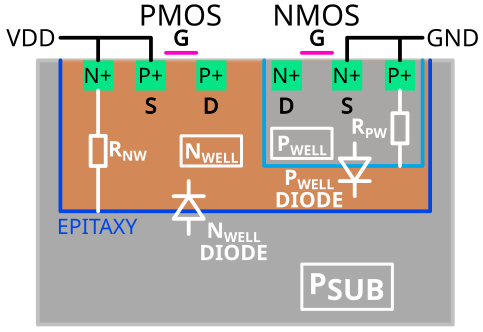
\includegraphics[width=7.8cm]{3_modeling/figures/TRIPLE.pdf}
        \caption{Triple-Well}
        \label{subfig:tripleIvx}
    \end{subfigure}
    \caption{Dual-well and triple-well inverter silicon sectional view.}
    \label{fig:dualTripleIvx}
\end{figure}
%On one hand, when performing EMFI (usually on the front side of the IC), air is the physical support to convey energy through electromagnetic waves.
%It is achieved by coupling the loop wire probe to the power delivery network loops.
%On the other hand, when working with BBI, the context is different.
%Indeed, the energy is conveyed through electrical charges through the silicon substrate.
%Therefore, the carriers have to go through the metallic probe and the whole substrate to reach the logic gates and the power delivery network in order to disturb the IC operation.
%Thus, the substrate type and design could have a significant impact on BBI efficiency.
%As a result, we explored and studied BBI in two specific scenarios depending on the substrate types: \dwF and \twF.
%Fig. \ref{fig:dualTripleIvx} shows the sectional views of two inverters manufactured in a \dwF and a \twF substrate respectively.
%These simple schematics are helpful in understanding the reasoning behind the design of the electrical models.
%
%Fig. \ref{subfig:dualIvx} depicts the cross-sectional view of a \dwF CMOS inverter.
%The P-doped silicon substrate is colored in gray, with $RC_{GND}$ being the access resistance from the epitaxy layer to the NMOS bulk.
%This physical environment is the conducting support of electrical charges which flow up to the NMOS transistor.
%The orange region is the N-doped silicon well, located inside the P-substrate to manufacture the PMOS transistors.
%$RC_{VDD}$ is the access resistance from the epitaxy to the PMOS bulk inside the $N_{WELL}$.
%In addition to the P-substrate, the N-well is the last environment electrical charges have to go through before reaching the PMOS transistor.
%
%Fig. \ref{subfig:tripleIvx} shows the cross-sectional view of a \twF CMOS inverter.
%As before, gray areas represent P-doped silicon, and orange areas N-doped silicon.
%$R_{NW}$ is the $N_{WELL}$ access resistance from the epitaxy to the PMOS bulk, and $R_{PW}$ is the $P_{WELL}$ access resistance from the $N_{WELL} - P_{WELL}$ junction to the NMOS bulk.
%In this case, two silicon junctions are present, represented by two independent diodes.
%In order to reach the PMOS transistors, charges have to go through the exact same environments as before.
%However, concerning NMOS transistors, they have to pass through two silicon junctions instead of none.
%As discussed in Chapter \ref{chap:5faultModel}, this has a significant impact on BBI induced effects.
%However, these schematics are incomplete and do not allow simulating ICs behaviors under BBI.
%
%Therefore, as it has been done in \cite{mathieuEMFI}, ICs are spatially split in elementary sections called standard-cells segments (SCS).
%However, in addition to the improvement of the \dwF proposed model proposed in \cite{mathieuEMFI}, we also introduce a \twF model in order to fully appreciate the behavioral differences of BBI applied to both substrate types.
%
%%\begin{figure}[ht]
    \centering
    \includegraphics[width=0.65\textwidth]{3_modeling/figures/substrateSubdivision_6.pdf}
    \caption{Substrate subdivision improvement over M. Dumont model for \emfi \cite{mathieuEMFI}. The backside is the accessible substrate, and the epitaxy is the highest substrate level, a.k.a. the silicon junction between the P-substrate and the N-well.}
    \label{fig:surfaceSubDivid}
\end{figure}
%%\begin{figure}[ht]
    \centering
    %\scriptsize
    % \setstretch{0.9}
    \begin{subfigure}{0.45\textwidth}
        % \def\svgwidth{9.0cm}
        \includegraphics[width=\textwidth]{3_modeling/figures/dualWell_no_5e.pdf}
        \caption{Dual-Well}
        \label{subfig:dualScs}
    \end{subfigure}
    \hfill
    \begin{subfigure}{0.45\textwidth}
        % \def\svgwidth{9.0cm}
        \includegraphics[width=\textwidth]{3_modeling/figures/tripleWell_no_5e.pdf}
        \caption{Triple-Well}
        \label{subfig:tripleScs}
    \end{subfigure}
    \caption{Three-dimensional Dual-Well and Triple-Well IC comprehensive standard-cell electrical schematic.}
    \label{fig:dualTripleScs}
\end{figure}
%The main improvement over the \dwF model proposed in \cite{mathieuEMFI} concerns the substrate resistive network, as shown in Fig. \ref{fig:surfaceSubDivid}.
%In \cite{mathieuEMFI}, the substrate network is coarse and only consists of six electrical resistances for each SCS.
%It means that they represent the entire SCS substrate thickness, width, and height (on the left in Fig \ref{fig:surfaceSubDivid}).
%Even though it is sufficient to appreciate the injection method effects while studying EMFI, mainly because the substrate is almost transparent when it comes to electromagnetic waves, but also because EMFI is mostly performed at the IC front side, it is not precise enough to model the spreading of he voltage pulse from the IC backside to the transistors.
%
%To that end, we decided to split as much as possible these resistors, as shown in Fig. \ref{fig:surfaceSubDivid}, to provide a precise enough substrate sub-model while keeping realistic computational workload.
%For the final models, it was decided to use an editable elementary thickness of $10 \; \mu m$, and fixed width and depth of $5 \; \mu m$ for each elementary six-resistors substrate models, according to the footprint of an SCS on the XY plane ($5 \; \mu m \; \times \; (6 \; \mu m \; \times \; 5 \; \mu m)$), resulting in a $30 \; \mu m$ wide and $5 \; \mu m$ deep SCS.
%One can remark that in Fig \ref{fig:dualTripleScs}, no number is given concerning the substrate thickness, as similar to LFI, it is an important parameter which does not have a fixed value.
%Indeed, an attacker may want to thin the substrate or not before performing BBI.
%
%Furthermore, as shown in Fig. \ref{fig:dualTripleScs}, both SCS models contain various electrical components describing the IC structure, roughly composed of:
%\begin{itemize}
%    \item Its substrate
%    \item Its silicon junction(s)
%    \item Its logic gates
%    \item Its power supply rails
%\end{itemize}
%These two models, while being close to each other, allow, thanks to their subtle differences, to properly consider the different behaviors each substrate type exhibits.
%In the next section, \dwF SCS model and \twF SCS model are consecutively considered and analyzed.
%
%\subsection{Standard-cell segment models \ddcold}
%\label{subSect:dualTripleWellScs}
%Historically, IC substrate was manufactured using an exclusive \dwF structure.
%However, nowadays, it is common to find on relatively modern ICs a mix of \dwF and \twF structures on a monolithic die.
%\twF substrate structures bring significant advantages over \dwF substrates.
%In digital ICs, it is mainly used to body bias transistors to optimize their performance under power constraints.
%When used in analog or mixed designs, it gives two main advantages: substrate cross-talk and noise reduction, in addition to power supply decoupling thanks to the additional P-N junction capacitance \cite{tripleWellDecoupling}.
%This is why we decided to cover \dwF and \twF structures in our models.
%
%Fig. \ref{subfig:dualScs} depicts an SCS \dwF model.
%Each significant section of the SCS is gray-framed and numbered:
%\begin{itemize}
%    \item The section \ovalbox{1} represents the substrate environment: resistive and isotropic.
%    \item The section \ovalbox{2} is the $P-N$ silicon junction between the P-substrate and the N-well, represented by a diode and its junction capacitance, in addition to an access resistance $RC-VDD$, being the N-well electrical resistance.
%    \item The section \ovalbox{3} is the substrate access resistance.
%    \item The sections \ovalbox{4P} and \ovalbox{4N} contain the average non-logical model of a hundred of logic gates.
%    \item The sections \ovalbox{5} and \ovalbox{5'} are the two levels of the power delivery network, which are low resistive metals.
%    \item The section \ovalbox{6} is the decoupling between both $GND$ and $V_{DD}$ power networks.
%\end{itemize}
%
%Fig. \ref{subfig:tripleScs} depicts the SCS \twF model as follows:
%\begin{itemize}
%    \item The section \ovalbox{2} is the $P-N$ silicon junction between the P-substrate and the N-well, represented by a diode and its junction capacitance, in addition to an access resistance $R_{NW}$, being the N-well electrical resistance.
%    \item The section \ovalbox{3} is the $N-P$ silicon junction between the N-well and the P-well, represented once again by a diode and its junction capacitance, in addition to an access resistance $R_{PW}$, being the P-well electrical resistance.
%    \item The sections \ovalbox{1}, \ovalbox{4P}, \ovalbox{4N}, \ovalbox{5'} and \ovalbox{6} being the same as before.
%\end{itemize}
%
%%\begin{figure}[H]
    \centering
    \includegraphics[width=0.5\textwidth]{3_modeling/figures/algoFigure5.png}
    \caption{Elementary substrate 3D netlist}
    \label{fig:algo}
\end{figure}
%\algdef{SE}% flags used internally to indicate we're defining a new block statement
[CLASS]% new block type, not to be confused with loops or if-statements
{Class}% "Class{name}" will indicate the start of the struct declaration
{EndClass}% "EndClass" ends the block indent
[1]% There is one argument, which is the name of the class
{\textbf{class} \textsc{#1}}% typesetting of the start of a struct
{\textbf{end class}}% typesetting the end of the struct

\algdef{SE}% flags used internally to indicate we're defining a new block statement
[METHOD]% new block type, not to be confused with loops or if-statements
{Method}% "Method{name}" will indicate the start of the struct declaration
{EndMethod}% "EndMethod" ends the block indent
[2]% There is one argument, which is the name of the data structure
{\textbf{method} \textsc{#1}}% typesetting of the start of a struct
{\textbf{end method}}% typesetting the end of the struct

\begin{figure}[H]
    \begin{Verbatim}[frame=single]
        .subckt elementary_bloc D F L R Re U
        R1 U N001 RH
        R2 N001 D RH
        R3 Re N001 RL
        R4 N001 F RL
        R5 N001 L RL
        R6 R N001 RL
        .ends elementary_bloc
    \end{Verbatim}
    \caption{Elementary substrate SPICE netlist}
    \label{fig:subSpiceNetlist}
\end{figure}

\begin{figure}[H]
    \begin{Verbatim}[frame=single]
    .subckt elementary_blocx6 D1 D2 D3 D4 D5 D6
    +F1 F2 F3 F4 F5 F6 L R RE1 RE2 RE3 RE4 RE5 RE6
    +U1 U2 U3 U4 U5 U6 VSUBCintC
    XX1 D1 F1 L VSUBCintL2 RE1 U1 elementary_bloc
    XX2 D2 F2 VSUBCintL2 VSUBCintL1 RE2 U2 elementary_bloc
    XX3 D3 F3 VSUBCintL1 VSUBCintC RE3 U3 elementary_bloc
    XX4 D4 F4 VSUBCintC VSUBCintR1 RE4 U4 elementary_bloc
    XX5 D5 F5 VSUBCintR1 VSUBCintR2 RE5 U5 elementary_bloc
    XX6 D6 F6 VSUBCintR2 R RE6 U6 elementary_bloc
    .ends elementary_blocx6
    \end{Verbatim}
    \caption{SCS substrate layer SPICE netlist}
    \label{fig:subSpiceSCS}
\end{figure}

%\begin{figure}[!h]
%    \begin{Verbatim}[frame=single]
%    R1 vic vlt Rmup/4
%    R2 vlt vi1c Rmup/4
%    RM1 vddc vlt RM1/4
%    Ra_TL1 vddc N001 Ra
%    Cdecp_L1 N001 gndc Cdecp
%    Cdecp_R1 vddc N002 Cdecp
%    Ra_BR1 N002 gndc Ra
%    RM2 gndc glb RM1/4
%    R3 gic glb Rmup/4
%    R4 glb gi1c Rmup/4
%    RM3 grb gndc RM1/4
%    RM4 vrt vddc RM1/4
%    R5 gic1 grb Rmup/4
%    R6 grb gi1c1 Rmup/4
%    R7 vrt vi1c1 Rmup/4
%    R8 vic1 vrt Rmup/4
%    vepi_curr vepi vepi_meas dc=0
%    Rn1 gndc ncgnmos RN
%    Rp1 vddc ncgpmos RP
%    cgp_n1 ncgnmos vgp cgp
%    cgn_n1 ncgnmos vepi_meas cgn
%    cgn_p1 ncgpmos vepi_meas cgn
%    cgp_p1 ncgpmos vgp cgp
%    RCVDD vddc vgp RcontactDW
%    CNWPS vgp vepi_meas cnw
%    RCGND gndc vepi_meas RcontactDW
%    xDNWPS vepi_meas vgp dnwps AREA=31.43u PJ=70u
%    \end{Verbatim}
%    \caption{Dual-well standard-cell upper section netlist}
%    \label{fig:SCSdualUp}
%\end{figure}
%
%\begin{figure}[!h]
%    \begin{Verbatim}[frame=single]
%    R1 vic vlt Rmup/4
%    R2 vlt vi1c Rmup/4
%    RM1 vddc vlt RM1/4
%    Ra_TL1 vddc N001 Ra
%    Cdecp_L1 N001 gndc Cdecp
%    Cdecp_R1 vddc N002 Cdecp
%    Ra_BR1 N002 gndc Ra
%    RM2 gndc glb RM1/4
%    R3 gic glb Rmup/4
%    R4 glb gi1c Rmup/4
%    RM3 grb gndc RM1/4
%    RM4 vrt vddc RM1/4
%    R5 gic1 grb Rmup/4
%    R6 grb gi1c1 Rmup/4
%    R7 vrt vi1c1 Rmup/4
%    R8 vic1 vrt Rmup/4
%    vepi_curr vepi vepi_meas dc=0
%    Rn1 gndc RNCN RN
%    Rp1 vddc RPCP RP
%    cgp_n1 VPsNw RNCN cgp
%    cgn_n1 RNCN VNwPw cgn
%    cgn_p1 RPCP VNwPw cgn
%    cgp_p1 VPsNw RPCP cgp
%    RNW1 VPsNw vddc RcontactTW
%    cnw1 VPsNw vepi_meas cnw
%    RPW1 gndc VNwPw RcontactTW
%    xdpsnw1 vepi_meas VPsNw dnwps AREA=15.72u PJ=40u
%    xdnwpw1 VNwPw VPsNw dnwps AREA=31.43u PJ=70u
%    cnw2 VNwPw VPsNw cnw
%    cnw3 VPsNw vepi_meas cnw
%    xdpsnw2 vepi_meas VPsNw dnwps AREA=15.72u PJ=40u
%    \end{Verbatim}
%    \caption{Dual-well standard-cell upper section netlist}
%    \label{fig:SCStripleUp}
%\end{figure}

%\begin{algorithm}[H]
%    \caption[ic algo func]{Generation algorithm classes and function}
%    \label{alg:genFuncClass}
%    \begin{algorithmic}
%        \Class{NetlistTextFile} \Comment{Object defining the netlist to be generated}
%        \State \textbf{text}: String content of the class
%        \State $write(value : String)$: Write characters into the parent class "\textbf{text}" attribute
%        \EndClass\\
%
%        \Class{DualWellSCS} \Comment{Dual-well standard-cell netlist}
%        \State \textbf{text}: String content of the class
%        \State $read()$: Read characters into the parent class "\textbf{text}" attribute
%        \EndClass\\
%
%        \Class{TripleWellSCS} \Comment{Triple-well standard-cell netlist}
%        \State \textbf{text}: String content of the class
%        \State $read()$: Read characters into the parent class "\textbf{text}" attribute
%        \EndClass\\
%
%        \Function{createNets}{X : float, Y : float, NET : String}
%        \State \Comment{Create nets to connect SCS together}
%        \State $NetArray \gets ???$
%        \State \Return NetArray
%        \EndFunction\\
%
%        \Function{writeInMainNetlist}{value : String}
%        \State \Comment{Write generated results into main netlist}
%        \State NetlistTextFile.write(value)
%        \EndFunction\\
%
%        \Function{subRHcalc}{ESUB : int, RH : float, RL : float}
%        \State \Comment{Calculate elementary substrate resistors}
%        \State $RH \gets RH \times (ESUB \div 10)$
%        \State $RL \gets RL \times (ESUB \div 10)$
%        \State \Return RH, RL
%        \EndFunction\\
%
%        \Function{SCSelemGen}{SUBTYPE} \Comment{Generate Standard Cell Segment Model}
%        \If{$SUBTYPE = DualWell$}
%        \State $SCSNetlistDW = DualWellSCS$
%        \State $SCSNetlistTW = None$
%        \ElsIf{$SUBTYPE = TripleWell$}
%        \State $SCSNetlistDW = None$
%        \State $SCSNetlistTW = TriplelWellSCS$
%        \ElsIf{$SUBTYPE = Mixed$}
%        \State $SCSNetlistDW = DualWellSCS$
%        \State $SCSNetlistTW = TriplelWellSCS$
%        \EndIf
%        \State $SCSNetlistArray \gets {SCSNetlistDW, SCSNetlistTW}$
%        \State \Return SCSNetlistArray
%        \EndFunction\\
%    \end{algorithmic}
%\end{algorithm}

\begin{algorithm}[H]
\caption[ic algo]{Integrated circuit SPICE netlist generation algorithm.}
\label{alg:icGen}
\begin{algorithmic}
    \Require SUBTYPE \Comment{IC substrate type: Dual-well, Triple-well, Mixed}
    \Require TSUB \Comment{IC substrate thickness}
    \Require ESUB \Comment{Elementary substrate block thickness}
    \Require VPUU \Comment{Voltage pulse amplitude}
    \Require PW \Comment{Voltage pulse width}
    \Require TFR \Comment{Voltage pulse rise and fall times}
    \Require SIMTIME \Comment{Simulation duration}
    \Require SIMSTEP \Comment{Simulation time step}
    \Require TEX \Comment{Desired X size (µm)}
    \Require TEY \Comment{Desired Y size (µm)}
    \State $RH \gets 2000$ \Comment{Elementary substrate up-down/front-rear resistor value}
    \State $RL \gets 500$ \Comment{Elementary substrate left-right resistor value}
    \State $WSEG \gets 30$
    \State $HSEG \gets 5$
    \State $W6SEG \gets 30 \div 6$
    \State $nC \gets TEX \div WSEG$ \Comment{Number of column}
    \State $nL \gets TEY \div HSEG$ \Comment{Number of lines}
    \State $nH \gets TSUB \div ESUB$ \Comment{Number of substrate layers}
    \Ensure nC, nL and nH are integers
%    \State $RH, RL \gets \Call{subRHcalc}{ESUB, RH, RL}$
    \State $RH \gets RH \times (ESUB \div 10)$ \Comment{Adjust RH value according to user defined variable}
    \State $RL \gets RL \times (ESUB \div 10)$ \Comment{Adjust RL value according to user defined variable}
    \ForAll{cY in [0; nL[}
        \ForAll{cX in [0; nH[}
            \State $\overrightarrow{X} \gets
            \left[\begin{array}{r}
                        cX \times WSEG\\
                        cX \times WSEG + 1 \times (W6SEG \div 2)\\
                        cX \times WSEG + 3 \times (W6SEG \div 2)\\
                        cX \times WSEG + 5 \times (W6SEG \div 2)\\
                        cX \times WSEG + 7 \times (W6SEG \div 2)\\
                        cX \times WSEG + 9 \times (W6SEG \div 2)\\
                        cX \times WSEG + 11 \times (W6SEG \div 2)\\
                        cX \times WSEG + 12 \times (W6SEG \div 2)\\
                \end{array}\right]$
            $;\overrightarrow{Y} \gets
            \left[\begin{array}{r}
                        cY \times HSEG\\
                        (cY + \frac{1}{2}) \times HSEG\\
                        (cY + 1) \times HSEG\\
                \end{array}\right]$
            \State $;\overrightarrow{P} \gets
            \left[\begin{array}{r}
                cY \times HSEG\\
                (cY + \frac{1}{2}) \times HSEG\\
                (cY + 1) \times HSEG\\
            \end{array}\right]$
        \EndFor
    \EndFor
    \State \textcolor{orange}{TO FINISH.}
\end{algorithmic}
\end{algorithm}

%Each area of the elementary SCS models were automatically generated using  a custom algorithm, shown in Alg. \ref{alg:icGen}.
%It was mainly designed in order to reduce as much as possible any human intervention to limit difficult to debug errors and inconsistencies.
%Furthermore, it provides a degree of flexibility due to the ease of user modifications directly into the generation algorithm parameters, as opposed to netlist editing, thereby reducing errors further.
%These models only represent a section of an integrated circuit. For effective use and verification, it is necessary to replicate and interconnect these models spatially as much as possible.
%This was accomplished by utilizing customized Python scripts coupled with procedural generation.
%The IC generation algorithm enables the modification of multiple settings to produce the desired outcomes, albeit with certain inherent structural limitations.
%Two of the main limitations are the fixed width and depth of the elementary SCS models, and the fixed number of metal levels in the power delivery network.
%On the contrary, the following is a non-exhaustive list of user-modifiable settings:
%\begin{itemize}
%	\item Global IC size.
%	\item Probe position.
%	\item IC global substrate thickness.
%	\item IC elementary substrate thickness.
%	\item Substrate type (\dwF, \twF, or mixed).
%	\item Voltage pulse amplitude.
%	\item Voltage pulse width.
%	\item Voltage pulse rise and fall times.
%	\item Simulation time and step.
%\end{itemize}
%Eventually, the generator script incorporates a visual inspection tool in order to quickly verify the correctness of the generated netlist.
%Alg. \ref{alg:icGen} shows the IC generation algorithm main function, which is to create the coordinates for every net in the netlist.
%%Alg. \ref{alg:icGen} presents the IC generation algorithm, alongside Fig. \ref{fig:algo}.
